\documentclass[aspectratio=169,11pt]{beamer}
\usetheme{Boadilla}
\usefonttheme{professionalfonts}
\usepackage{amsmath,amssymb,booktabs,array,multirow}
\usepackage{tikz}
\usetikzlibrary{arrows.meta,positioning,shapes.geometric,fit,calc}
\usepackage{ragged2e}
\usepackage{xcolor}
\usepackage{tabularx}
\usepackage{adjustbox}
\usepackage{hyperref}
\setbeamertemplate{navigation symbols}{}
\setbeamertemplate{footline}[frame number]
\setbeamertemplate{itemize item}{\small$\blacktriangleright$}
\setbeamertemplate{itemize subitem}{\scriptsize$\bullet$}
\definecolor{IITblue}{RGB}{30,64,100}
\definecolor{IITlight}{RGB}{232,239,247}
\definecolor{IITgold}{RGB}{180,130,35}
\definecolor{Deep}{RGB}{35,35,35}
\definecolor{Green}{RGB}{55,110,75}
\setbeamercolor{structure}{fg=IITblue}
\setbeamercolor{frametitle}{fg=IITblue}
\setbeamercolor{title}{fg=IITblue}
\setbeamercolor{block title}{fg=white,bg=IITblue}
\setbeamercolor{block body}{bg=IITlight!55!white}
\setbeamercolor{alerted text}{fg=IITgold}
\setlength{\parskip}{3pt}
\newcommand{\smallcaps}[1]{\textsc{#1}}
\newcommand{\key}[1]{\textbf{\color{IITblue}#1}}
\newcommand{\sourcefoot}[1]{\vfill\tiny\color{gray}Source: Task Force Proposal, September 2026. #1}
\newcommand{\sectorbox}[2]{\begin{block}{#1}\small #2\end{block}}

\title{Enhancing Core-Sector Employment and Career Pathways\\for IIT Bombay Chemical Engineering B.Tech Students}
\subtitle{Departmental Presentation of the Task Force Proposal}
\author{Profs. Sanjay Mahajani (Head), Abhijit Majumder, Jyoti Seth,  Rahul Nabar, Sameer Jadhav,  Madhu Vinjamur, Yogendra Shastri, Rochish M. Thaokar}
\institute{Department of Chemical Engineering\\Indian Institute of Technology Bombay}
\date{October 2026}

\begin{document}

\begin{frame}
  \titlepage
\end{frame}

\begin{frame}{Purpose of today's discussion}
\begin{itemize}
\item This is not a proposal to ``force'' students into traditional Chemical Engineering jobs.
\item It is an attempt to ask a more fundamental question: \key{How can Chemical Engineering become an employer-of-choice ecosystem for our strongest students?}
\item The proposed intervention acts simultaneously on three sides:
  \begin{enumerate}
  \item \key{Prepare better students} for technologically demanding roles.
  \item \key{Create better roles} that genuinely use IIT Bombay capability.
  \item \key{Build deeper industry relationships} beyond annual placement transactions.
  \end{enumerate}
\item The intended outcome is a sustainable \key{student--industry--alumni ecosystem}, not merely a larger recruiter count.
\end{itemize}
\sourcefoot{}
\end{frame}

\section{I. Why a Task Force?}
\begin{frame}{The central challenge}
\begin{block}{The observation}
Chemical Engineering at IIT Bombay provides a strong foundation in mathematics, physical sciences, engineering science, transport phenomena, thermodynamics, reaction engineering and process systems. Yet an increasing proportion of strong undergraduate students choose career pathways outside the traditional Chemical Engineering ecosystem.
\end{block}
\vspace{4mm}
\begin{center}
\Large\key{How do we make Chemical Engineering and its associated industries an employer of choice for our strongest undergraduate talent?}
\end{center}
\vspace{3mm}
\begin{itemize}
\item This is not simply a question of increasing the number of companies at placements.
\item The target is \key{high-quality, technically challenging, well-compensated and upwardly mobile careers}.
\end{itemize}
\sourcefoot{Proposal pp. 2--3.}
\end{frame}

\begin{frame}{What has changed in the Chemical Engineering opportunity space?}
\begin{columns}[T]
\column{0.48\textwidth}
\begin{block}{Traditional perception}
\begin{itemize}
\item Refineries
\item Petrochemicals
\item Chemical manufacturing
\item Plant operations
\item Production engineering
\end{itemize}
\end{block}
\column{0.48\textwidth}
\begin{block}{Expanding ecosystem}
\begin{itemize}
\item Advanced materials
\item Semiconductors and electronic chemicals
\item Pharma / biopharma
\item Specialty and fine chemicals
\item New energy, batteries, hydrogen
\item Carbon capture / circular economy
\item Automation, computational engineering, AI/ML
\item High-end R\&D, technology management
\item Deep-tech entrepreneurship
\end{itemize}
\end{block}
\end{columns}
\vspace{3mm}
\centering\large\key{The question is not whether the Chemical Engineering ecosystem is shrinking; it is whether we are connecting our students to its expanding frontier.}
\end{frame}

\begin{frame}{A potentially self-reinforcing, sub-optimal equilibrium}
\centering
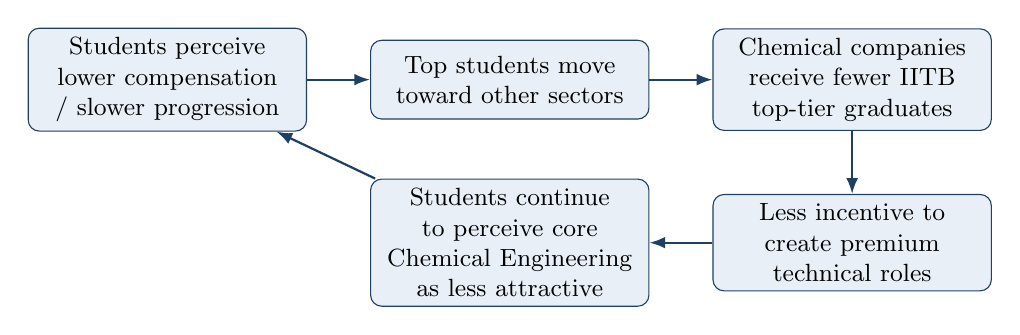
\begin{tikzpicture}[node distance=8mm and 8mm, every node/.style={font=\small}, box/.style={draw=IITblue,rounded corners,fill=IITlight,align=center,text width=3.3cm,minimum height=1.0cm}, arr/.style={-{Latex[length=2mm]},thick,IITblue}]
\node[box] (s) {Students perceive lower compensation / slower progression};
\node[box,right=of s] (t) {Top students move toward other sectors};
\node[box,right=of t] (c) {Chemical companies receive fewer IITB top-tier graduates};
\node[box,below=of c] (i) {Less incentive to create premium technical roles};
\node[box,left=of i] (p) {Students continue to perceive core Chemical Engineering as less attractive};
\draw[-{Latex[length=2mm]},thick,IITblue] (s)--(t); \draw[-{Latex[length=2mm]},thick,IITblue] (t)--(c); \draw[-{Latex[length=2mm]},thick,IITblue] (c)--(i); \draw[-{Latex[length=2mm]},thick,IITblue] (i)--(p); \draw[-{Latex[length=2mm]},thick,IITblue] (p)--(s);
\end{tikzpicture}
\vspace{5mm}
\begin{alertblock}{Task Force response}
Break the cycle from both ends: \key{student capability} + \key{industry role creation}.
\end{alertblock}
\sourcefoot{Proposal pp. 3--4.}
\end{frame}

\begin{frame}{Exposure alone is not enough}
\begin{center}
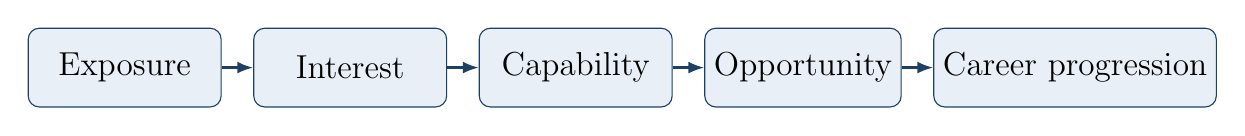
\begin{tikzpicture}[node distance=4mm, every node/.style={font=\large}, stp/.style={draw=IITblue,rounded corners,fill=IITlight,minimum width=2.45cm,minimum height=1.0cm,align=center}, arr/.style={-{Latex[length=2mm]},thick}]
\node[stp] (a) {Exposure};\node[stp,right=of a] (b) {Interest};\node[stp,right=of b] (c) {Capability};\node[stp,right=of c] (d) {Opportunity};\node[stp,right=of d] (e) {Career progression};
\draw[-{Latex[length=2mm]},thick,IITblue] (a)--(b);\draw[-{Latex[length=2mm]},thick,IITblue] (b)--(c);\draw[-{Latex[length=2mm]},thick,IITblue] (c)--(d);\draw[-{Latex[length=2mm]},thick,IITblue] (d)--(e);
\end{tikzpicture}
\end{center}
\vspace{6mm}
\begin{columns}[T]
\column{0.48\textwidth}
\begin{itemize}
\item More lectures, visits and company presentations are useful.
\item But exposure by itself is unlikely to change career choices substantially.
\end{itemize}
\column{0.48\textwidth}
\begin{block}{Where the Task Force concentrates}
\key{Capability} and \key{Opportunity}: students must be prepared for valuable roles, and industry must see those roles as worth creating.
\end{block}
\end{columns}
\end{frame}

\begin{frame}{The proposition to industry}
\begin{block}{Do not hire an IIT Bombay Chemical Engineer merely as a better production engineer.}
Create roles that leverage IIT-level analytical, computational and technological capability.
\end{block}
\vspace{4mm}
\begin{columns}[T]
\column{0.48\textwidth}
\textbf{Examples of high-value roles}
\begin{itemize}
\item Technical services
\item R\&D / process development
\item Technology development
\item Projects
\item Process control / digitalisation
\item AI/ML / simulation
\end{itemize}
\column{0.48\textwidth}
\begin{itemize}
\item New-energy technology
\item Advanced materials
\item Technical strategy / technology management
\item Technical consulting
\item CEO/CTO technology offices
\item Deep-tech entrepreneurship
\end{itemize}
\end{columns}
\sourcefoot{Proposal pp. 4, 12.}
\end{frame}

\begin{frame}{Chemical Engineering as a platform, not a narrow track}
\begin{center}
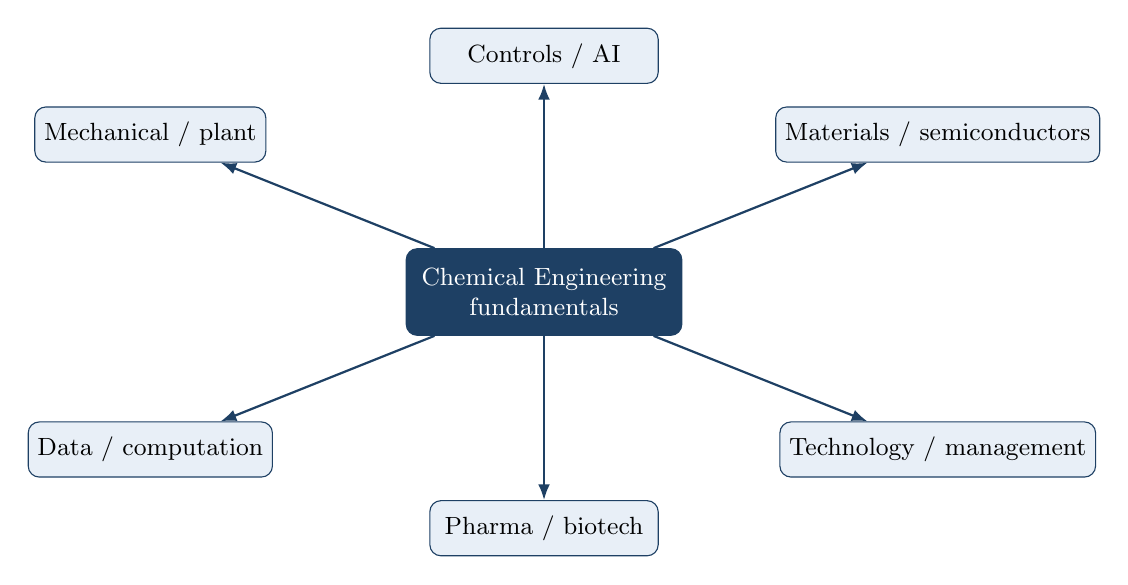
\begin{tikzpicture}[every node/.style={font=\small}, core/.style={draw=IITblue,fill=IITblue,text=white,rounded corners,minimum width=3.5cm,minimum height=1.1cm,align=center}, outbox/.style={draw=IITblue,fill=IITlight,rounded corners,minimum width=2.9cm,minimum height=0.7cm,align=center}]
\node[core] (ce) at (0,0) {Chemical Engineering\\fundamentals};
\node[outbox] (me) at (-5,2) {Mechanical / plant};
\node[outbox] (el) at (0,3) {Controls / AI};
\node[outbox] (mat) at (5,2) {Materials / semiconductors};
\node[outbox] (ds) at (-5,-2) {Data / computation};
\node[outbox] (ph) at (0,-3) {Pharma / biotech};
\node[outbox] (mg) at (5,-2) {Technology / management};
\foreach \x in {me,el,mat,ds,ph,mg}{\draw[-{Latex[length=2mm]},thick,IITblue] (ce)--(\x);}
\end{tikzpicture}
\end{center}
\vspace{2mm}
\centering\key{Strong quantitative and engineering foundations can open careers traditionally occupied by several disciplines.}
\end{frame}

\section{II. Objectives and Architecture}
\begin{frame}{Six objectives of the Task Force}
\begin{enumerate}
\item \key{Increase high-quality core-sector opportunities} — quality, diversity and technical depth, not recruiter count alone.
\item \key{Improve the quality of roles} — shift toward process engineering, R\&D, technology, digitalisation, controls, AI/ML, projects and advanced technical functions.
\item \key{Create a student-to-industry pipeline} — early exposure → internship → Practice School / DDP → PPO / placement.
\item \key{Align curriculum and skills with industry needs} through formal sector-wise skill maps.
\item \key{Build long-term strategic industry relationships} beyond annual placements.
\item \key{Establish Chemical Engineering as a platform for multiple high-value careers}, including research and entrepreneurship.
\end{enumerate}
\end{frame}

\begin{frame}{The complete architecture}
\centering
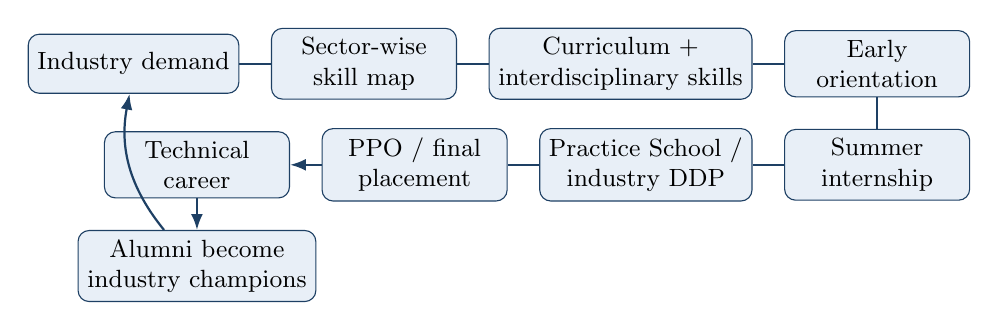
\begin{tikzpicture}[node distance=4mm, every node/.style={font=\small}, box/.style={draw=IITblue,fill=IITlight,rounded corners,align=center,minimum width=2.35cm,minimum height=0.75cm}, arr/.style={-{Latex[length=2mm]},thick,IITblue}]
\node[box] (d) {Industry demand};
\node[box,right=of d] (m) {Sector-wise\\skill map};
\node[box,right=of m] (c) {Curriculum +\\interdisciplinary skills};
\node[box,right=of c] (e) {Early\\orientation};
\node[box,below=of e] (i) {Summer\\internship};
\node[box,left=of i] (ps) {Practice School /\\industry DDP};
\node[box,left=of ps] (p) {PPO / final\\placement};
\node[box,left=of p] (tc) {Technical\\career};
\draw[-{Latex[length=2mm]},thick,IITblue] (d)--(m)--(c)--(e)--(i)--(ps)--(p)--(tc);
\node[box,below=of tc] (al) {Alumni become\\industry champions};
\draw[-{Latex[length=2mm]},thick,IITblue] (tc)--(al);
\draw[-{Latex[length=2mm]},thick,IITblue] (al) to[bend left=25] (d);
\end{tikzpicture}
\vspace{3mm}
\begin{alertblock}{Long-term objective}
A self-reinforcing \key{Chemical Engineering Industry--Talent Ecosystem at IIT Bombay}.
\end{alertblock}
\end{frame}

\begin{frame}{The student-to-industry pipeline}
\begin{center}
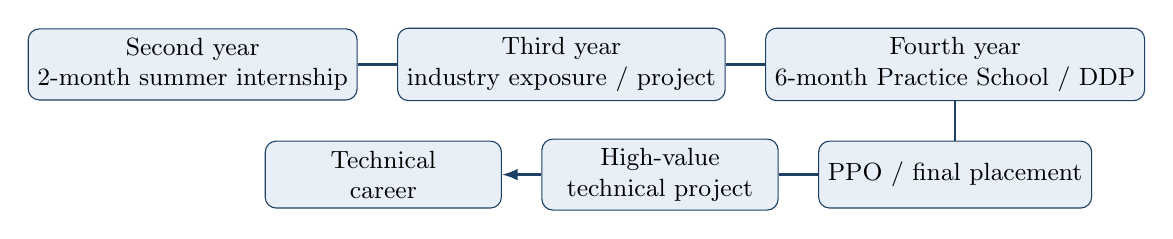
\begin{tikzpicture}[node distance=5mm, every node/.style={font=\small}, stp/.style={draw=IITblue,fill=IITlight,rounded corners,minimum width=3.0cm,minimum height=0.85cm,align=center}, arr/.style={-{Latex[length=2mm]},thick}]
\node[stp] (y2) {Second year\\2-month summer internship};
\node[stp,right=of y2] (y3) {Third year\\industry exposure / project};
\node[stp,right=of y3] (y4) {Fourth year\\6-month Practice School / DDP};
\node[stp,below=of y4] (ppo) {PPO / final placement};
\node[stp,left=of ppo] (tech) {High-value\\technical project};
\node[stp,left=of tech] (career) {Technical\\career};
\draw[-{Latex[length=2mm]},thick,IITblue] (y2)--(y3)--(y4)--(ppo)--(tech)--(career);
\end{tikzpicture}
\end{center}
\vspace{4mm}
\begin{itemize}
\item Internship is not an isolated summer activity; it becomes part of recruitment strategy.
\item The relationship evolves from exposure to demonstrated capability to a career decision.
\item A strong industry mentor is essential for maintaining technical relevance.
\end{itemize}
\end{frame}

\section{III. Opportunity Landscape}
\begin{frame}{The opportunity map: sectors to be systematically explored}
\begin{columns}[T]
\column{0.5\textwidth}
\begin{itemize}
\item Oil, gas, refining and petrochemicals
\item Specialty and fine chemicals
\item Pharmaceuticals and biotechnology
\item FMCG and consumer products
\item Semiconductors and electronic materials
\item New energy and sustainability
\item Process control, automation and industrial digitalisation
\end{itemize}
\column{0.5\textwidth}
\begin{itemize}
\item EPC, engineering and projects
\item Materials and computational engineering
\item Biomedical devices / BiomedTech
\item Startups and entrepreneurship
\item International engineering careers
\item Research / PhD / advanced technology
\item AI/ML across the Chemical Engineering ecosystem
\end{itemize}
\end{columns}
\vspace{3mm}
\centering\large\key{Every sector needs an industry map, role map, skill map and engagement plan.}
\end{frame}

\begin{frame}{Sector 1 — Oil, Gas, Refining and Petrochemicals}
\begin{columns}[T]
\column{0.49\textwidth}
\textbf{Industry space}
\begin{itemize}
\item Exploration and production; refineries; petrochemicals; LNG; gas processing
\item Specialty petroleum products; process technology; oilfield technology; digital oilfield
\item Global companies, Indian majors and PSUs
\end{itemize}
\column{0.49\textwidth}
\textbf{Target roles}
\begin{itemize}
\item Process / design / technical services
\item Process optimisation and simulation
\item R\&D and technology development
\item Advanced control / digital process engineering
\item Energy optimisation, process safety, projects
\end{itemize}
\end{columns}
\vspace{3mm}
\begin{block}{Strategic emphasis}
For IIT Bombay students, prioritise technical services, R\&D, process engineering, technology, projects, optimisation, advanced control and digitalisation rather than primarily retail, generic marketing or non-technical roles.
\end{block}
\end{frame}

\begin{frame}{Sector 2 — Specialty and Fine Chemicals}
\begin{columns}[T]
\column{0.46\textwidth}
\textbf{Potential targets}
\begin{itemize}
\item UPL
\item Aarti Industries
\item Atul
\item DCM Shriram
\item Birla Group companies
\item Other specialty/fine chemical companies
\end{itemize}
\column{0.5\textwidth}
\textbf{Potential roles}
\begin{itemize}
\item Process development / intensification
\item R\&D and scale-up
\item Process safety / technology development
\item Plant optimisation / technical services
\item Projects / digitalisation / AI
\item Sustainability / new product development
\end{itemize}
\end{columns}
\vspace{3mm}
\begin{alertblock}{Key challenge}
Many mid-sized firms may not automatically create IITB-level roles. The Task Force should work with them to \key{design roles around IITB capabilities}.
\end{alertblock}
\end{frame}

\begin{frame}{Sector 3 — Pharmaceuticals and Biotechnology}
\begin{columns}[T]
\column{0.5\textwidth}
\textbf{Industry segments}
\begin{itemize}
\item Pharmaceutical manufacturing
\item Process development
\item Biopharmaceuticals / bioprocessing
\item Drug delivery / formulation
\item Fermentation / continuous manufacturing
\item Biotechnology and BiomedTech startups
\end{itemize}
\column{0.47\textwidth}
\textbf{Roles for Chemical Engineers}
\begin{itemize}
\item Process / bioprocess engineering
\item R\&D and scale-up
\item Manufacturing technology
\item Formulation / continuous processing
\item Data/analytics and process control
\item Technology transfer
\end{itemize}
\end{columns}
\vspace{3mm}
\centering\key{Chemistry + Biology + Engineering + Data is an important interdisciplinary space.}
\end{frame}

\begin{frame}{Sector 4 — FMCG and Consumer Products}
\begin{columns}[T]
\column{0.48\textwidth}
\textbf{Potential targets}
\begin{itemize}
\item Hindustan Unilever
\item Procter \& Gamble
\item Other major FMCG companies
\end{itemize}
\column{0.48\textwidth}
\textbf{Potential roles}
\begin{itemize}
\item Process engineering / manufacturing technology
\item Product development / R\&D
\item Supply-chain analytics
\item Sustainability / packaging / materials
\item Data / AI
\item Executive / leadership associate
\item Technology management
\end{itemize}
\end{columns}
\vspace{4mm}
\begin{block}{Specific action}
Investigate UFLP-type programmes and executive-associate pathways and communicate them clearly to students.
\end{block}
\end{frame}

\begin{frame}{Sector 5 — Semiconductors and Electronic Materials}
\begin{block}{Why this matters}
Semiconductor manufacturing is highly skill-intensive and combines technicians, process engineers, materials experts, chemical engineers, process-control specialists, data analysts and PhD-level researchers.
\end{block}
\begin{columns}[T]
\column{0.48\textwidth}
\textbf{Chemical Engineering roles}
\begin{itemize}
\item Semiconductor / wafer process engineering
\item Wet chemical processing
\item Deposition / etching / cleaning
\item CMP
\item Ultra-high-purity chemicals
\item Contamination control
\end{itemize}
\column{0.48\textwidth}
\begin{itemize}
\item Process optimisation / control
\item Materials development
\item Manufacturing analytics
\item DDPs and summer internships
\item Six-month Practice School
\item Industry-embedded PhD opportunities
\end{itemize}
\end{columns}
\end{frame}

\begin{frame}{Semiconductor strategy — from interest to capability}
\begin{enumerate}
\item Develop semiconductor-oriented electives / modules.
\item Establish DDP projects with semiconductor companies.
\item Develop two-month summer internships.
\item Develop six-month Practice School opportunities.
\item Explore industry-embedded PhD programmes.
\item Engage Tata Electronics and other semiconductor organisations.
\item Build relationships with semiconductor-industry leadership and alumni.
\item Participate in relevant industry events and campus initiatives.
\item Obtain a formal skill-requirement map from companies.
\end{enumerate}
\begin{block}{Immediate questions to industry}
Current hiring needs? Future skills? Appropriate ChemE roles? Internship/Practice School/DDP possibilities? International opportunities?
\end{block}
\end{frame}

\begin{frame}{Sector 6 — New Energy, Energy Transition and Sustainability}
\begin{columns}[T]
\column{0.47\textwidth}
\begin{itemize}
\item Hydrogen / green hydrogen
\item Fuel cells
\item Batteries / energy storage
\item Carbon capture / utilisation
\item Biofuels / sustainable fuels
\item Renewable-energy systems
\end{itemize}
\column{0.47\textwidth}
\begin{itemize}
\item Circular economy / waste-to-energy
\item Process decarbonisation
\item Energy systems
\item Battery process engineering
\item Hydrogen systems
\item Carbon management
\item AI/ML for energy systems
\end{itemize}
\end{columns}
\vspace{5mm}
\begin{block}{Proposed trajectory}
Thermodynamics + Transport + Reaction Engineering + Electrochemistry + Materials + Process Systems + AI/ML + Energy Systems.
\end{block}
\end{frame}

\begin{frame}{Sector 7 — Process Control, Automation and Industrial Digitalisation}
\begin{columns}[T]
\column{0.49\textwidth}
\textbf{Potential employers}
\begin{itemize}
\item Automation / process-control companies
\item Industrial digitalisation companies
\item Energy / chemical companies
\item EPC organisations
\item Semiconductor manufacturers
\end{itemize}
\column{0.49\textwidth}
\textbf{Potential roles}
\begin{itemize}
\item Process / advanced process control
\item Automation engineering
\item Digital twins
\item Process optimisation
\item Industrial AI / analytics
\item Predictive maintenance
\item Model-based control
\end{itemize}
\end{columns}
\vspace{5mm}
\centering\Large\key{Chemical Engineering + Controls + AI}\par
\vspace{2mm}\normalsize can become a major differentiator for IIT Bombay graduates.
\end{frame}

\begin{frame}{Sector 8 — EPC, Engineering and Projects}
\begin{columns}[T]
\column{0.48\textwidth}
\textbf{Potential targets}
\begin{itemize}
\item Larsen \& Toubro
\item Toyo Engineering
\item Jacobs
\item Engineers India
\item Other EPC / engineering organisations
\end{itemize}
\column{0.48\textwidth}
\textbf{Potential roles}
\begin{itemize}
\item Process design / simulation
\item Plant design / process safety
\item Project engineering / management
\item Digital engineering
\item Technology development
\end{itemize}
\end{columns}
\vspace{5mm}
\begin{center}
\small Process Engineer $\rightarrow$ Senior Engineer $\rightarrow$ Project Engineer $\rightarrow$ Project Manager $\rightarrow$ Technology/Engineering Manager $\rightarrow$ Technical/Business Leadership
\end{center}
\end{frame}

\begin{frame}{Sector 9 — Materials and Computational Engineering}
\begin{columns}[T]
\column{0.48\textwidth}
\textbf{Areas}
\begin{itemize}
\item Materials informatics
\item Molecular simulation
\item Computational chemistry
\item Process simulation
\item Multiscale modelling
\item Battery / semiconductor materials
\item Polymers / advanced materials
\end{itemize}
\column{0.48\textwidth}
\textbf{Roles}
\begin{itemize}
\item Computational scientist
\item Materials scientist
\item Simulation engineer
\item AI/ML engineer
\item Materials informatics scientist
\item R\&D scientist
\end{itemize}
\end{columns}
\end{frame}

\begin{frame}{Sector 10 — Biomedical Devices and BiomedTech}
\begin{block}{Potential areas}
Medical devices; drug delivery; biomaterials; diagnostics; microfluidics; bioprocessing; biomedical startups.
\end{block}
\vspace{5mm}
\begin{center}
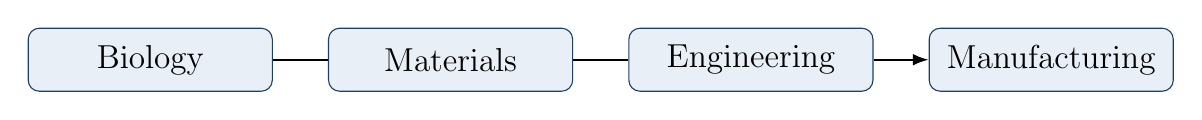
\begin{tikzpicture}[node distance=7mm, every node/.style={font=\large}, b/.style={draw=IITblue,fill=IITlight,rounded corners,minimum width=3.1cm,minimum height=0.8cm,align=center}]
\node[b] (bio) {Biology};\node[b,right=of bio] (mat) {Materials};\node[b,right=of mat] (eng) {Engineering};\node[b,right=of eng] (man) {Manufacturing};
\draw[-{Latex[length=2mm]},thick] (bio)--(mat)--(eng)--(man);
\end{tikzpicture}
\end{center}
\vspace{4mm}
\centering\key{Appropriate electives + research + industry projects can position ChemE students at this interface.}
\end{frame}

\begin{frame}{Sector 11 — Startups and Entrepreneurship}
\begin{columns}[T]
\column{0.48\textwidth}
\textbf{Target areas}
\begin{itemize}
\item Climate technology / energy
\item Batteries / hydrogen / carbon capture
\item Biotechnology / medtech
\item Advanced materials
\item Industrial AI / process automation
\item Semiconductor technology
\end{itemize}
\column{0.48\textwidth}
\textbf{Potential roles}
\begin{itemize}
\item Technical co-founder
\item R\&D / product development
\item Founder's / Technical Founder's Office
\item Technology strategy
\item Process development
\item Product management
\end{itemize}
\end{columns}
\vspace{4mm}
\begin{block}{Why this matters for exceptional students}
A founder's-office or technical-founder pathway can be a highly attractive alternative to conventional entry-level employment.
\end{block}
\end{frame}

\begin{frame}{Research and PhD as a deliberate career pathway}
\centering
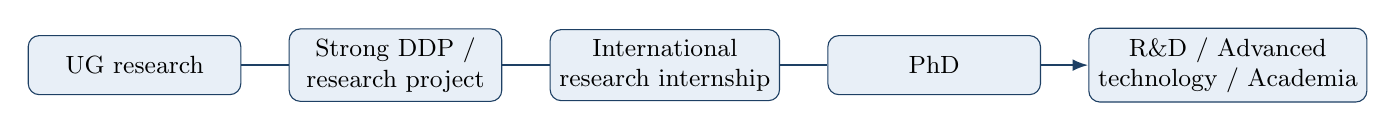
\begin{tikzpicture}[node distance=6mm, every node/.style={font=\small}, s/.style={draw=IITblue,fill=IITlight,rounded corners,minimum width=2.7cm,minimum height=.75cm,align=center},a/.style={-{Latex[length=2mm]},thick}]
\node[s] (ug) {UG research};\node[s,right=of ug] (ddp) {Strong DDP /\\research project};\node[s,right=of ddp] (int) {International\\research internship};\node[s,right=of int] (phd) {PhD};\node[s,right=of phd] (r) {R\&D / Advanced\\technology / Academia};
\draw[-{Latex[length=2mm]},thick,IITblue] (ug)--(ddp)--(int)--(phd)--(r);
\end{tikzpicture}
\vspace{5mm}
\begin{itemize}
\item Particularly important for semiconductors, materials, biotechnology, energy, computational science, AI/ML and advanced processes.
\item Students need guidance on strong PhD applications, course selection, research projects and international internships.
\item Research orientation should be viewed as a legitimate high-value career pathway—not as a residual option.
\end{itemize}
\end{frame}

\begin{frame}{International opportunities}
\begin{columns}[T]
\column{0.48\textwidth}
\textbf{Potential channels}
\begin{itemize}
\item IIT Bombay Chemical Engineering alumni
\item Multinational companies
\item International R\&D laboratories
\item International universities
\item Semiconductor / energy companies
\item Japanese, US and European organisations
\end{itemize}
\column{0.48\textwidth}
\textbf{Potential geographies}
\begin{itemize}
\item USA
\item Europe
\item Japan
\item Singapore
\item Middle East
\end{itemize}
\vspace{2mm}
Map alumni willing to support internships, research projects, industry projects and international recruitment.
\end{columns}
\end{frame}

\section{IV. What Roles Can Our Students Target?}
\begin{frame}{Role taxonomy — the opportunity is broader than ``core''}
\begin{columns}[T]
\column{0.5\textwidth}
\textbf{Core technical}
\begin{itemize}
\item Process / design / development
\item Technical services
\item Process safety / scale-up
\item Plant optimisation / projects
\end{itemize}
\textbf{R\&D / scientific}
\begin{itemize}
\item R\&D scientist / research engineer
\item Materials / computational scientist
\item Product development
\end{itemize}
\textbf{Digital / AI}
\begin{itemize}
\item AI/ML / industrial AI
\item Process data science
\item Digital twins / optimisation
\end{itemize}
\column{0.5\textwidth}
\textbf{Controls}
\begin{itemize}
\item Process / advanced process control
\item Automation / MPC
\end{itemize}
\textbf{Technology / strategy}
\begin{itemize}
\item Technology / engineering / programme management
\item CEO / CTO / Founder's Office
\item Technology scouting / consulting
\end{itemize}
\textbf{Technical-commercial / entrepreneurship / research}
\begin{itemize}
\item Product management / technical marketing / technical sales
\item Deep-tech founder / startup R\&D
\item Direct PhD / research assistant / international research
\end{itemize}
\end{columns}
\end{frame}

\begin{frame}{Career relevance of foundational Chemical Engineering courses}
\begin{tabularx}{\textwidth}{>{\bfseries}p{3.2cm} X}
\toprule
Foundation & Examples of future-facing application \\
\midrule
Mathematics & Process modelling, optimisation, data-driven engineering \\
Thermodynamics & Energy systems, separations, hydrogen, batteries \\
Transport phenomena & Semiconductor processing, materials, microfluidics \\
Reaction engineering & Pharma, fuels, specialty chemicals, energy \\
Process dynamics & Automation, advanced control, digitalisation \\
Materials & Batteries, semiconductors, advanced materials \\
AI / computation & Process optimisation, digital twins, materials discovery \\
\bottomrule
\end{tabularx}
\vspace{4mm}
\centering\key{Early students should see where the fundamentals they learn are used in real technology.}
\end{frame}

\section{V. Student Development and Curriculum}
\begin{frame}{Start early — second year, not placement season}
\begin{block}{Question students should be able to answer early}
What does a Chemical Engineer actually do in ExxonMobil, Tata Electronics, UPL, Unilever, a semiconductor fab, a battery company, a startup or an R\&D laboratory?
\end{block}
\begin{itemize}
\item Use practising engineers, scientists and technology leaders—not only faculty—for early exposure.
\item Embed career context in core second-year courses.
\item Develop sector-specific pathways before students reach placement season.
\item Make the relationship between fundamentals and technology careers explicit.
\end{itemize}
\end{frame}

\begin{frame}{Industry Skill $\rightarrow$ Curriculum Mapping}
\scriptsize
\begin{tabularx}{\textwidth}{>{\bfseries}p{2.2cm} p{3.1cm} p{4.0cm} X}
\toprule
Sector & Core knowledge & Advanced skills & Additional skills \\
\midrule
Oil \& Gas & Thermo, transport, reaction & Simulation, optimisation & AI/ML \\
Pharma & Reaction, transport & Bioprocess, formulation & Data analytics \\
Semiconductor & Transport, materials & Process technology & Controls, materials \\
Controls & Process dynamics & APC, MPC & AI/ML \\
New Energy & Thermo, electrochemistry & Batteries, hydrogen & Modelling \\
Specialty chemicals & Reaction, separations & Scale-up, process development & AI \\
EPC & Core ChemE & Simulation, design & Project management \\
Materials & Thermo, transport & Materials simulation & ML \\
FMCG & Core ChemE & Product/process development & Analytics \\
\bottomrule
\end{tabularx}
\vspace{2mm}
\centering\key{This mapping should be validated through direct industry consultation.}
\end{frame}

\begin{frame}{Potential elective / module portfolio}
\begin{columns}[T]
\column{0.5\textwidth}
\begin{itemize}
\item Advanced Process Control
\item AI/ML for Chemical Engineering
\item Process Systems Engineering
\item Semiconductor Processing
\item Pharmaceutical Engineering
\item Bioprocess Engineering
\item New Energy Technologies
\item Electrochemical Engineering
\end{itemize}
\column{0.5\textwidth}
\begin{itemize}
\item Battery Technology
\item Hydrogen Technology
\item Materials Simulation
\item Computational Chemical Engineering
\item Industrial Data Analytics
\item Digital Twins
\item Sustainability Engineering
\end{itemize}
\end{columns}
\vspace{4mm}
\begin{alertblock}{Important qualification}
The objective is \key{not} necessarily to create a large number of new courses. Strengthen existing courses and create interdisciplinary trajectories wherever possible.
\end{alertblock}
\end{frame}

\section{VI. Industry Engagement}
\begin{frame}{From placement interaction to strategic partnership}
\begin{center}
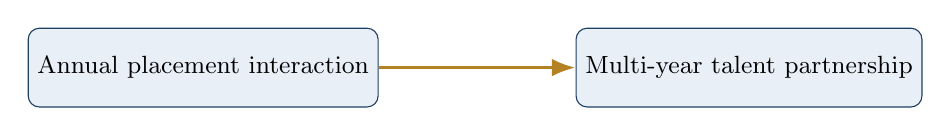
\begin{tikzpicture}[node distance=8mm, every node/.style={font=\small}, box/.style={draw=IITblue,fill=IITlight,rounded corners,minimum width=4.0cm,minimum height=1.0cm,align=center}]
\node[box] (old) {Annual placement interaction};
\node[box,right=25mm of old] (new) {Multi-year talent partnership};
\draw[-{Latex[length=3mm]},very thick,IITgold] (old)--(new);
\end{tikzpicture}
\end{center}
\vspace{5mm}
\begin{columns}[T]
\column{0.48\textwidth}
\textbf{Possible components}
\begin{itemize}
\item Sponsored research
\item Industry-defined DDPs
\item Internships / Practice School
\item Guest lectures / industrial courses
\item Faculty visits
\end{itemize}
\column{0.48\textwidth}
\begin{itemize}
\item Industry advisory boards
\item PhD programmes
\item R\&D collaborations
\item International opportunities
\item Recruitment
\end{itemize}
\end{columns}
\end{frame}

\begin{frame}{Questions for CEO / CTO / R\&D / Engineering leadership}
\begin{enumerate}
\item What roles are expected to grow?
\item What skills are currently missing in fresh IIT graduates?
\item Which roles can B.Tech Chemical Engineers occupy?
\item What prevents the company from hiring more IITB Chemical Engineers?
\item What would justify higher compensation?
\item What internship projects would be useful?
\item Can the company provide DDP projects?
\item Can it provide six-month Practice School positions?
\item Can internships convert into PPOs?
\item Can projects be jointly defined with IITB faculty?
\item What skills will be required five years from now?
\end{enumerate}
\vspace{2mm}
\centering\key{These answers should drive the skill map and not the other way around.}
\end{frame}

\begin{frame}{Industry engagement hierarchy}
\centering
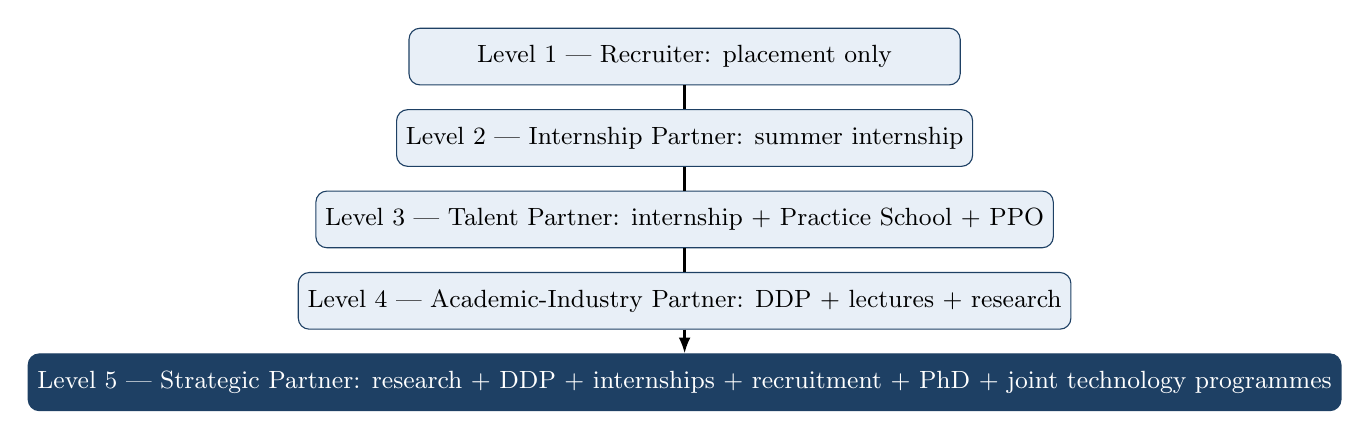
\begin{tikzpicture}[node distance=3mm, every node/.style={font=\small}, l/.style={draw=IITblue,rounded corners,fill=IITlight,minimum width=7.0cm,minimum height=.72cm,align=center}]
\node[l] (1) {Level 1 — Recruiter: placement only};
\node[l,below=of 1] (2) {Level 2 — Internship Partner: summer internship};
\node[l,below=of 2] (3) {Level 3 — Talent Partner: internship + Practice School + PPO};
\node[l,below=of 3] (4) {Level 4 — Academic-Industry Partner: DDP + lectures + research};
\node[l,below=of 4,fill=IITblue,text=white] (5) {Level 5 — Strategic Partner: research + DDP + internships + recruitment + PhD + joint technology programmes};
\draw[-{Latex[length=2mm]},thick] (1)--(2)--(3)--(4)--(5);
\end{tikzpicture}
\vspace{3mm}
\centering\key{Move selected high-potential companies progressively up the engagement ladder.}
\end{frame}

\begin{frame}{Industry-defined DDP programme}
\begin{block}{Basic model}
Industry provides a portfolio of real technical problems; IIT Bombay provides faculty supervision and strong students.
\end{block}
\begin{columns}[T]
\column{0.48\textwidth}
\begin{itemize}
\item Process optimisation
\item Energy reduction
\item Waste minimisation
\item Digital twins
\item AI-based process monitoring
\item New process development
\end{itemize}
\column{0.48\textwidth}
\begin{itemize}
\item Scale-up
\item Semiconductor process optimisation
\item Battery manufacturing
\item Carbon capture
\item Advanced materials
\item Process control
\end{itemize}
\end{columns}
\vspace{3mm}
\begin{center}\Large\key{Industry Mentor + IITB Faculty Mentor + Student}\end{center}
\end{frame}

\begin{frame}{Six-month Practice School / apprenticeship}
\begin{itemize}
\item A major strategic intervention: expand six-month industry engagements to a significant fraction of interested B.Tech students.
\item Priority sectors: PSUs, semiconductors, pharma, specialty chemicals, EPC, new energy and controls.
\item A PPO cannot necessarily be guaranteed, especially in PSUs.
\item But a strong Practice School experience can improve both recruitment quality and career matching.
\end{itemize}
\vspace{5mm}
\begin{block}{Principle}
The six-month engagement should be treated as an \key{educational and technical experience}, not simply as an extended internship.
\end{block}
\end{frame}

\begin{frame}{Mentor-based industry model}
\begin{center}
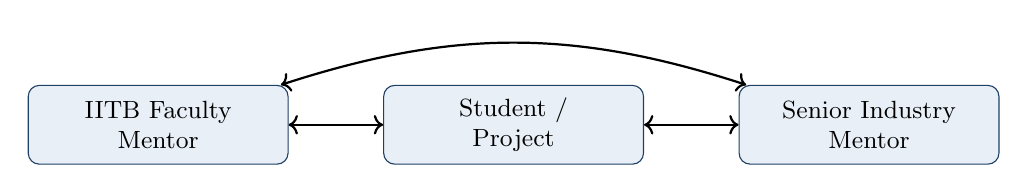
\begin{tikzpicture}[node distance=12mm, every node/.style={font=\small}, b/.style={draw=IITblue,fill=IITlight,rounded corners,minimum width=3.3cm,minimum height=1cm,align=center}]
\node[b] (f) {IITB Faculty\\Mentor};\node[b,right=of f] (s) {Student /\\Project};\node[b,right=of s] (i) {Senior Industry\\Mentor};
\draw[<->,thick] (f)--(s);\draw[<->,thick] (s)--(i);\draw[<->,thick] (f) to[bend left=18] (i);
\end{tikzpicture}
\end{center}
\vspace{5mm}
\begin{itemize}
\item Industry mentor should ideally be a senior engineer, R\&D scientist, technology manager or project leader—not only an HR contact.
\item Expected benefits: project quality, learning, industry engagement, assessment, PPO decisions and long-term relationships.
\end{itemize}
\end{frame}

\section{VII. Industry-Specific Strategies}
\begin{frame}{Large multinationals and giants}
\begin{block}{Examples}
ExxonMobil, Shell, Reliance, Unilever, P\&G, Schlumberger and large pharmaceutical companies.
\end{block}
\textbf{Challenge:} global recruitment structures may not create positions specifically for IIT Bombay Chemical Engineering.
\vspace{3mm}
\textbf{Strategy}
\begin{itemize}
\item Engage global and India R\&D heads.
\item Engage GCC leadership and identify technical roles.
\item Seek international internships and DDP pipelines.
\item Build global alumni champions.
\item Explore global mobility.
\end{itemize}
\end{frame}

\begin{frame}{PSUs — use technical depth, not just conventional recruitment}
\begin{columns}[T]
\column{0.47\textwidth}
\textbf{Strengths}
\begin{itemize}
\item Stability and long-term careers
\item Strong technical infrastructure
\item Large engineering operations
\item R\&D capability
\end{itemize}
\textbf{Challenges}
\begin{itemize}
\item PPO may not be available
\item Rigid recruitment structures
\item IITB talent may not be distinguished by conventional channels
\end{itemize}
\column{0.49\textwidth}
\textbf{Strategic focus}
\begin{itemize}
\item R\&D
\item Technical services
\item Process engineering
\item Technology development
\item Projects
\item Advanced process control
\end{itemize}
\vspace{3mm}
Senior faculty/alumni should connect directly with Heads, Directors, R\&D and Refinery leadership—not rely exclusively on HR.
\end{columns}
\end{frame}

\begin{frame}{Mid-sized chemical companies — potentially the largest untapped opportunity}
\begin{block}{Potential targets}
UPL, Aarti Industries, Atul, DCM Shriram, Birla Group companies and other specialty chemical firms.
\end{block}
\begin{columns}[T]
\column{0.48\textwidth}
\textbf{Barriers}
\begin{itemize}
\item Salary differential
\item Perception of hierarchical/subordinate roles
\item Attrition concerns
\item Limited graduate programmes
\item Lack of clearly defined IIT-level roles
\end{itemize}
\column{0.48\textwidth}
\textbf{Possible roles}
\begin{itemize}
\item Technology development
\item Process innovation / optimisation
\item R\&D / new product development
\item Digitalisation / AI/ML
\item Sustainability / special projects
\item CEO/CTO technical advisor
\end{itemize}
\end{columns}
\end{frame}

\begin{frame}{A critical industry proposition: value before compensation}
\begin{block}{The wrong proposition}
``Convince chemical companies to pay IITB salaries.''
\end{block}
\begin{block}{The stronger proposition}
``Help IITB graduates create enough additional value that chemical companies want to pay IITB salaries.''
\end{block}
\vspace{4mm}
\begin{columns}[T]
\column{0.48\textwidth}
\begin{itemize}
\item Quantitative ability
\item Process simulation
\item AI/ML
\item Advanced optimisation
\item Multiphysics modelling
\end{itemize}
\column{0.48\textwidth}
\begin{itemize}
\item Experimental capability
\item Process innovation
\item Cross-disciplinary engineering
\item Technology development
\item Leadership
\end{itemize}
\end{columns}
\sourcefoot{Proposal pp. 49, 64--65.}
\end{frame}

\begin{frame}{Startups — a different value proposition}
\begin{itemize}
\item Startups can provide broader responsibility and direct exposure to technology development.
\item Create structured startup internships and startup DDPs.
\item Organise founder interaction sessions.
\item Develop faculty--startup projects.
\item Explore technical co-founder pathways.
\item Use the IIT Bombay entrepreneurship ecosystem where appropriate.
\end{itemize}
\vspace{5mm}
\centering\Large\key{For exceptional students, ownership and learning velocity may be as important as the conventional job title.}
\end{frame}

\section{VIII. Industry Feedback and Friction Points}
\begin{frame}{Why industry feedback matters}
\begin{block}{A key methodological point}
The Task Force should not redesign curriculum based only on faculty intuition. It should first understand what industry is actually experiencing: hiring constraints, skill gaps, attrition, role design, compensation and career progression.
\end{block}
\begin{itemize}
\item The proposal records candid feedback from DRL, TRDDC/TCS, former UPL context, Aarti Industries and sector-specific discussions.
\item These are not universal claims; they are \key{inputs to be tested and quantified} through a systematic industry survey.
\end{itemize}
\end{frame}

\begin{frame}{Industry feedback — practical friction points}
\scriptsize
\begin{tabularx}{\textwidth}{>{\bfseries}p{2.5cm} X X}
\toprule
Organisation / context & Feedback recorded & Implication for Task Force \\
\midrule
Dr. Reddy's Laboratories & Attrition within 1--2 years; need for stronger hands-on laboratory preparation; hesitation toward field-based experimental tasks; recruitment through online case-study challenges. & Improve practical preparation; build a structured training/internship relationship; understand retention and career expectations. \\
TRDDC / TCS & High-impact R\&D but entry compensation reported at 12--14 LPA, limiting IITB attractiveness. & Understand compensation/value mismatch; identify roles where IITB capability can be differentiated. \\
Ex-UPL context & Process-sector value is realised over longer deployment cycles; finance/HR constraints on premium engineering packages; plant geography affects attraction. & Role design, visible technical contribution, career progression and facility quality matter. \\
Aarti Industries & Distinct advanced technical-service / problem-solving cadres; 15--20 LPA suggested target for fresh IITB talent; structured rotation and accelerated leadership trajectories discussed. & Explore technically differentiated cadres, rotation and progression models. \\
\bottomrule
\end{tabularx}
\sourcefoot{Recorded industry discussions in proposal, pp. 66--68.}
\end{frame}

\begin{frame}{Sector-specific feedback already available}
\begin{itemize}
\item \key{Semiconductors:} integrate introductory ChemE fundamentals early; use Unit Operations industry lectures across second, third and fourth years; leverage sector events and alumni leaders.
\item \key{PSUs / Oil \& Gas:} direct leadership outreach to refinery/PSU directors; redirect recruitment toward R\&D and technical services; prioritise second-year internships and Practice School.
\item \key{FMCG / Unilever:} investigate structured UFLP recruitment, CEO Executive Associate routes, basic-sciences recruitment and entrepreneurship support.
\item \key{Research orientation:} provide structured mentoring for students preparing PhD applications, with attention to course selection and undergraduate research.
\item \key{Emerging areas:} process intensification, advanced effluent treatment, green technology, food engineering and related technology opportunities should be explored.
\end{itemize}
\sourcefoot{Proposal pp. 67--68.}
\end{frame}

\section{IX. Alumni, Faculty and Sector Teams}
\begin{frame}{Alumni as a strategic resource}
\begin{block}{Build an alumni database by}
Company • sector • country • function • seniority • R\&D • technical services • engineering • management • CEO/CTO • entrepreneurship
\end{block}
\vspace{4mm}
\begin{itemize}
\item First approach should preferably be through an alumni champion inside the organisation.
\item A respected IITB Chemical Engineering alumnus can be substantially more effective than a cold approach through generic channels.
\item Alumni can support internships, research, DDPs, Practice School, international opportunities and recruitment.
\item Successful alumni should become the next generation of \key{industry champions}.
\end{itemize}
\end{frame}

\begin{frame}{Proposed sector responsibility structure}
\scriptsize
\begin{tabularx}{\textwidth}{>{\bfseries}p{4.0cm} p{3.2cm} X}
\toprule
Sector & Faculty lead / team & Principal deliverable \\
\midrule
Semiconductors & Sunthar / Rochish & Skill map, DDPs, Practice School, Tata Electronics links, industry PhD \\
Biomedical / BiomedTech & Mahesh & Target firms/startups; microfluidics, biomaterials, bioprocess trajectory \\
Controls / Automation / AI & Sharad & Employer directory; international placements; AI/ML trajectory \\
Pharma / Biotech & Sarika / Pramod & Structured internship pipelines; technical career pathways \\
New Energy / Sustainability & Yogendra & Hydrogen, batteries, carbon capture, decarbonisation; DDPs \\
Oil \& Gas / PSU & Aloke / Sanjay & Leadership outreach; R\&D/technical services pathways \\
Specialty Chemicals & Task Force team & Company mapping and role creation \\
FMCG & Task Force team & Targeted leadership / programme pathways \\
EPC / Projects & Task Force team & Technical role and project pipeline \\
International & Alumni / Task Force & Alumni mapping and overseas opportunities \\
Entrepreneurship & Task Force + IITB ecosystem & Startup pathways \\
\bottomrule
\end{tabularx}
\end{frame}

\begin{frame}{Sector dossier — the standard deliverable}
\begin{enumerate}
\item \key{Industry map:} giants, PSUs, mid-sized firms, startups, international companies.
\item \key{Roles:} 10--15 specific roles appropriate for IITB Chemical Engineering graduates.
\item \key{Skill requirements:} curriculum coverage, missing skills, electives, software/computation, laboratory/research skills.
\item \key{Industry contacts:} CEO, CTO, R\&D Head, Engineering Head, HR and IITB alumni.
\item \key{Engagement opportunities:} lectures, internships, Practice School, DDP, sponsored projects, PhD, placement, international internship.
\item \key{Recruitment potential:} High / Medium / Low.
\item \key{Action plan:} responsible faculty/member, industry contact, first action, expected outcome, timeline.
\end{enumerate}
\vspace{3mm}
\centering\key{A sector dossier is more useful than a static company list.}
\end{frame}

\section{X. Immediate and Medium-Term Plan}
\begin{frame}{Immediate action plan — 2026--27}
\begin{enumerate}
\item Build the industry map.
\item Obtain industry skill maps.
\item Secure immediate internships in semiconductor, pharma, specialty chemicals, oil/gas, controls, new energy and R\&D.
\item Build the Practice School pipeline.
\item Build an initial portfolio of 20--30 industry-defined DDP topics.
\item Increase senior industry lectures, technical workshops and mentoring.
\item Launch an alumni campaign and identify Sector Champions.
\end{enumerate}
\vspace{3mm}
\begin{block}{Scale of initial industry database}
Approximately 20--30 major companies + 30--50 mid-sized companies + 15--20 startups + 10--15 international opportunities.
\end{block}
\end{frame}

\begin{frame}{Immediate actions already specified in the proposal}
\begin{itemize}
\item Identify senior graduates across target organisations as Sector Champions.
\item Initiate direct discussions with PSU Directors and Refinery Leadership.
\item Engage with relevant semiconductor campus initiatives and senior alumni.
\item Launch two-month second-year summer internships and six-month Practice School placements across priority sectors.
\item Formalise a dedicated training partnership with Dr. Reddy's Laboratories, responding to feedback on practical laboratory preparation.
\item Embed practical career context in core second-year coursework.
\item Organise specialised Unit Operations guest lectures by industry practitioners for second-, third- and fourth-year cohorts.
\end{itemize}
\sourcefoot{Proposal pp. 53--55.}
\end{frame}

\begin{frame}{Medium-term plan — 2027--28}
\begin{columns}[T]
\column{0.32\textwidth}
\begin{block}{Curriculum}
\begin{itemize}
\item Skill-gap analysis
\item Develop/modify electives
\item Interdisciplinary offerings
\end{itemize}
\end{block}
\column{0.32\textwidth}
\begin{block}{Students}
\begin{itemize}
\item Sector trajectories
\item AI/ML pathway
\item Semiconductor pathway
\item New energy pathway
\item Pharma/biotech
\item Controls
\end{itemize}
\end{block}
\column{0.32\textwidth}
\begin{block}{Industry}
\begin{itemize}
\item Expand internships
\item Expand DDPs
\item Practice School partners
\item Industry mentors
\end{itemize}
\end{block}
\end{columns}
\vspace{5mm}
\centering\key{The first year should establish evidence and relationships; the second year institutionalises the pathways.}
\end{frame}

\begin{frame}{Long-term vision — 2028 onwards}
\begin{itemize}
\item \key{Industry Advisory Board} spanning oil/gas, specialty chemicals, pharma, semiconductors, energy, FMCG, controls, EPC and startups.
\item \key{Industry-linked curriculum} with selected courses/modules jointly informed by industry.
\item \key{Industry-embedded DDP programme} with a substantial real-problem portfolio.
\item \key{Permanent Practice School network}.
\item \key{Industry-sponsored laboratories} in semiconductors, AI/ML, process control, new energy and advanced materials.
\item \key{Industry PhD programmes} in technology-intensive sectors.
\item \key{International engagement} through systematic alumni outreach.
\item \key{Undergraduate research track} for competitive global PhD pathways.
\end{itemize}
\end{frame}

\begin{frame}{Timeline}
\scriptsize
\begin{tabularx}{\textwidth}{>{\bfseries}p{3.0cm} X}
\toprule
Period & Major action \\
\midrule
Q3--Q4 2026 & Industry mapping; alumni mapping; CEO/CTO/R\&D dialogues; immediate internships \\
Q4 2026 & Identify industry mentors \\
Q4 2026--Q1 2027 & Obtain industry skill maps \\
Q1--Q2 2027 & Curriculum / skill-gap analysis; expand Practice School and DDP partnerships; develop student trajectories \\
Q2--Q3 2027 & Develop / modify electives \\
Q3--Q4 2027 & Pilot enhanced internship / DDP model \\
2027--28 & Expand industry partnerships \\
2028--29 & Full implementation \\
2028 onward & Continuous industry partnership and outcome assessment \\
\bottomrule
\end{tabularx}
\end{frame}

\section{XI. Measurement and Governance}
\begin{frame}{How should we measure success?}
\begin{block}{Not just total placement numbers}
The dashboard should measure the quality and depth of the Chemical Engineering ecosystem.
\end{block}
\begin{columns}[T]
\column{0.48\textwidth}
\textbf{Employment}
\begin{itemize}
\item Core recruiters / offers
\item Technical / R\&D offers
\item High-value roles
\item International offers
\end{itemize}
\textbf{Internships}
\begin{itemize}
\item Summer internships
\item Practice School
\item Industry DDPs
\item PPOs
\item International internships
\end{itemize}
\column{0.48\textwidth}
\textbf{Industry engagement}
\begin{itemize}
\item Active partners
\item Senior interactions
\item Mentors
\item Industry-defined projects
\item Sponsored research
\end{itemize}
\textbf{Student capability}
\begin{itemize}
\item Sector trajectories
\item AI/ML participation
\item Industry R\&D
\item International internships
\item UG research / PhD
\end{itemize}
\end{columns}
\end{frame}

\begin{frame}{The most important outcome metric}
\begin{center}
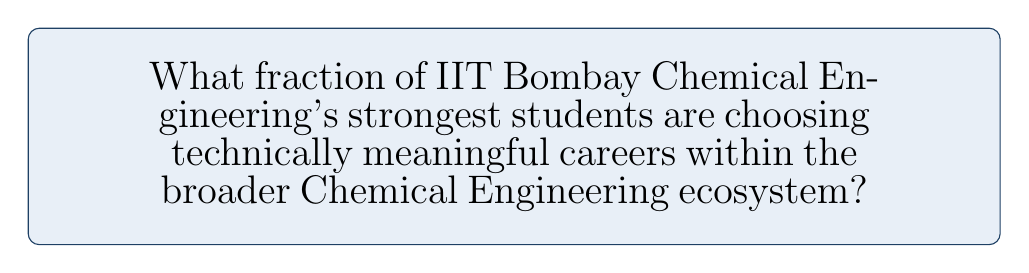
\begin{tikzpicture}
\node[draw=IITblue,fill=IITlight,rounded corners,inner sep=12pt,text width=11.5cm,align=center] {
\Large What fraction of IIT Bombay Chemical Engineering's strongest students are choosing technically meaningful careers within the broader Chemical Engineering ecosystem?
};
\end{tikzpicture}
\end{center}
\vspace{7mm}
\begin{itemize}
\item This captures \key{quality of employment}, not merely quantity.
\item The broader ecosystem deliberately includes energy, semiconductors, materials, pharma, digitalisation, AI/ML, advanced manufacturing, R\&D, entrepreneurship and research.
\item A successful intervention should improve both \key{student capability} and \key{industry demand for that capability}.
\end{itemize}
\end{frame}

\begin{frame}{Fundamental principles}
\begin{enumerate}
\item \key{Quality over quantity} — high-quality technical career opportunities matter more than recruiter count.
\item \key{Exposure is necessary but insufficient} — exposure must lead to capability, opportunity and career.
\item \key{Industry before curriculum redesign} — understand current and future needs first.
\item \key{Industry must create appropriate roles} — use quantitative, engineering, computational and research capabilities.
\item \key{Students must create demonstrable value} — capability must justify premium opportunity.
\item \key{Start early} — second year, not placement season.
\item \key{Build relationships, not transactions} — Research + Curriculum + Internship + DDP + Practice School + Recruitment + Alumni.
\end{enumerate}
\end{frame}

\section{XII. What This Means for the Department}
\begin{frame}{What changes inside the Department?}
\begin{columns}[T]
\column{0.48\textwidth}
\textbf{For students}
\begin{itemize}
\item Earlier career orientation
\item Sector trajectories
\item More industry-linked projects
\item Better practical preparation
\item Stronger computation / AI / interdisciplinary capability
\item Research pathway
\end{itemize}
\textbf{For curriculum}
\begin{itemize}
\item Evidence-based skill mapping
\item Strengthen existing offerings
\item Targeted new electives/modules
\end{itemize}
\column{0.48\textwidth}
\textbf{For faculty}
\begin{itemize}
\item Sector responsibility
\item Industry mentors and visits
\item Industry-defined projects
\item Sponsored research
\item Alumni engagement
\end{itemize}
\textbf{For industry relations}
\begin{itemize}
\item Named partners and champions
\item Multi-year engagement
\item DDP / Practice School pipeline
\item Technical—not only HR—relationships
\end{itemize}
\end{columns}
\end{frame}

\begin{frame}{What we should avoid}
\begin{itemize}
\item \key{Do not} equate employability with more placement companies alone.
\item \key{Do not} equate ``core'' with only refinery / petrochemical / plant operations.
\item \key{Do not} create electives without first establishing demand and student uptake.
\item \key{Do not} depend exclusively on HR or annual placement visits for industry relationships.
\item \key{Do not} assume that compensation can be improved without demonstrable additional value.
\item \key{Do not} treat internships, DDPs and Practice School as disconnected activities.
\item \key{Do not} make every student follow the same career path.
\item \key{Do not} neglect research, international careers, startups or technology-management trajectories.
\end{itemize}
\end{frame}

\begin{frame}{What we should build instead}
\begin{center}
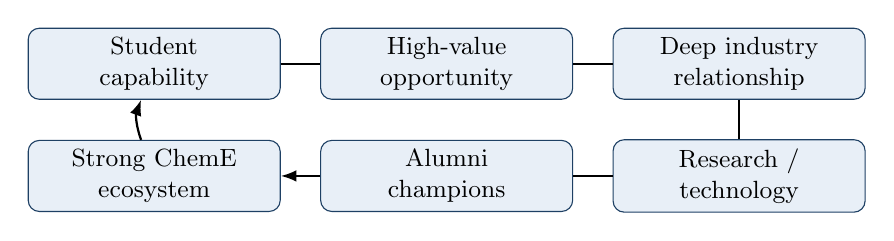
\begin{tikzpicture}[node distance=5mm, every node/.style={font=\small}, b/.style={draw=IITblue,fill=IITlight,rounded corners,minimum width=3.2cm,minimum height=.8cm,align=center}]
\node[b] (cap) {Student\\capability};
\node[b,right=of cap] (opp) {High-value\\opportunity};
\node[b,right=of opp] (rel) {Deep industry\\relationship};
\node[b,below=of rel] (res) {Research /\\technology};
\node[b,left=of res] (al) {Alumni\\champions};
\node[b,left=of al] (eco) {Strong ChemE\\ecosystem};
\draw[-{Latex[length=2mm]},thick] (cap)--(opp)--(rel)--(res)--(al)--(eco);
\draw[-{Latex[length=2mm]},thick] (eco) to[bend left=20] (cap);
\end{tikzpicture}
\end{center}
\vspace{6mm}
\centering\Large\key{A virtuous cycle rather than a placement-season intervention.}
\end{frame}

\begin{frame}{A possible departmental operating model}
\begin{enumerate}
\item \key{Task Force core} — coordinate, monitor, maintain database and dashboard.
\item \key{Sector teams} — each owns a sector dossier and industry relationship pipeline.
\item \key{Alumni champions} — open doors and provide organisational intelligence.
\item \key{Faculty mentors} — connect industry problems to academic capability.
\item \key{Industry mentors} — define meaningful problems and assess student performance.
\item \key{Students} — build demonstrable technical capability through courses, projects and internships.
\item \key{Department} — periodically review outcomes and adjust priorities based on evidence.
\end{enumerate}
\vspace{4mm}
\begin{block}{Governance principle}
The Task Force should be a \key{living system for evidence and relationships}, not a one-time report.
\end{block}
\end{frame}

\section{XIII. Discussion and Departmental Decisions}
\begin{frame}{Questions for the Department}
\begin{enumerate}
\item Do we agree that the objective is \key{quality and breadth of technical careers}, rather than simply more recruiters?
\item Which sectors should receive the first wave of faculty attention?
\item Can we identify faculty/teams willing to own sector dossiers?
\item How aggressively should we expand second-year internships and six-month Practice School?
\item What industry-defined DDP mechanism can we operationalise quickly?
\item Which existing courses can immediately incorporate career/industry context?
\item Which skill gaps require new electives, and which can be addressed through existing courses/modules?
\item How should the Department systematically engage alumni?
\item What data should become part of an annual employability dashboard?
\item What institutional support is required from IIT Bombay beyond the Department?
\end{enumerate}
\end{frame}

\begin{frame}{The first 90 days — a practical starting point}
\begin{columns}[T]
\column{0.31\textwidth}
\begin{block}{Month 1}
\begin{itemize}
\item Finalise sector teams
\item Start industry database
\item Map alumni champions
\item Identify immediate internship leads
\end{itemize}
\end{block}
\column{0.31\textwidth}
\begin{block}{Month 2}
\begin{itemize}
\item CEO/CTO/R\&D dialogues
\item Collect skill requirements
\item Identify DDP problems
\item Identify Practice School partners
\end{itemize}
\end{block}
\column{0.31\textwidth}
\begin{block}{Month 3}
\begin{itemize}
\item Produce sector dossiers
\item Launch industry lectures
\item Secure first internship/DDP cohort
\item Establish dashboard
\end{itemize}
\end{block}
\end{columns}
\vspace{5mm}
\centering\key{Begin with relationships and evidence; curriculum reform follows from what we learn.}
\end{frame}

\begin{frame}{Concluding vision}
\begin{block}{The objective is not to persuade students to remain in ``traditional core Chemical Engineering.''}
The objective is to redefine and expand the Chemical Engineering opportunity space so that IIT Bombay graduates can occupy high-value technical, scientific, technological and leadership positions across the evolving chemical-engineering ecosystem.
\end{block}
\vspace{4mm}
\begin{itemize}
\item Refinery
\item Specialty chemicals
\item Semiconductor fab
\item Pharmaceutical R\&D centre
\item Battery / hydrogen company
\item Advanced materials laboratory
\item AI-driven process company
\item EPC organisation
\item Global R\&D centre
\item Deep-tech startup
\end{itemize}
\end{frame}

\begin{frame}{The common thread}
\begin{center}
\Large\key{The common thread is not the industry label.}
\vspace{6mm}
\Large It is the ability to apply
\vspace{2mm}
\Large engineering fundamentals + quantitative reasoning + computation + experimentation + AI + interdisciplinary thinking
\vspace{4mm}
\Large to technologically important problems.
\end{center}
\vspace{6mm}
\begin{block}{Our proposition to students}
We will help you become demonstrably better prepared for the technological problems of the next generation.
\end{block}
\end{frame}

\begin{frame}{The proposition to industry}
\begin{center}
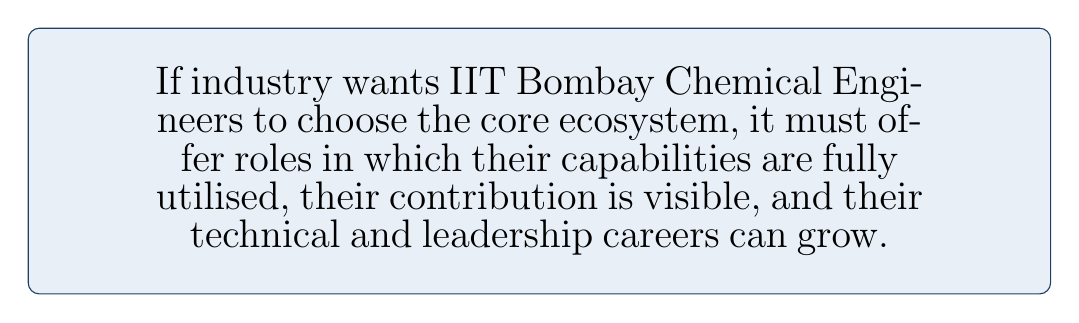
\begin{tikzpicture}
\node[draw=IITblue,fill=IITlight,rounded corners,inner sep=14pt,text width=12cm,align=center] {
\Large If industry wants IIT Bombay Chemical Engineers to choose the core ecosystem, it must offer roles in which their capabilities are fully utilised, their contribution is visible, and their technical and leadership careers can grow.
};
\end{tikzpicture}
\end{center}
\vspace{7mm}
\begin{center}
\Large\key{Prepare better students. \quad Create better roles. \quad Build deeper industry relationships.}
\end{center}
\end{frame}

\begin{frame}{From a placement problem to a talent-development opportunity}
\begin{center}
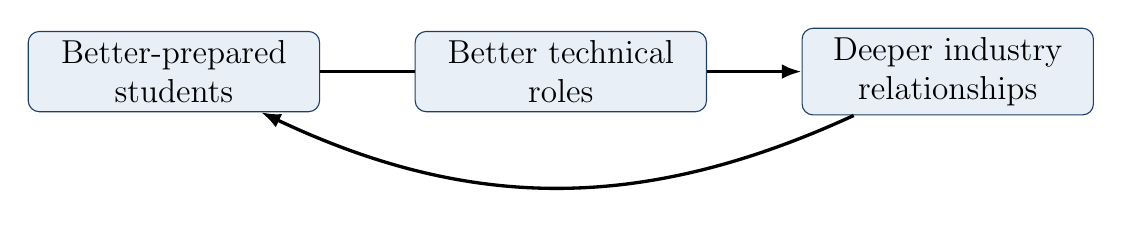
\begin{tikzpicture}[node distance=12mm, every node/.style={font=\large}, b/.style={draw=IITblue,fill=IITlight,rounded corners,minimum width=3.7cm,minimum height=1cm,align=center}]
\node[b] (s) {Better-prepared\\students};
\node[b,right=of s] (r) {Better technical\\roles};
\node[b,right=of r] (i) {Deeper industry\\relationships};
\draw[-{Latex[length=2.5mm]},very thick] (s)--(r)--(i);
\draw[-{Latex[length=2.5mm]},very thick] (i) to[bend left=25] (s);
\end{tikzpicture}
\end{center}
\vspace{8mm}
\begin{center}
\Huge\color{IITblue}\textbf{Chemical Engineering}\par
\vspace{2mm}
\Large\textbf{as a platform for the next generation of technology careers}
\end{center}
\end{frame}

\begin{frame}[plain]
\centering
\vspace{2cm}
{\Huge\color{IITblue}\textbf{Thank you}}\\[8mm]
{\Large Discussion and suggestions from the Department}
\vfill
\small Task Force Proposal — Chemical Engineering Department, IIT Bombay — September 2026
\end{frame}

\end{document}
